\section{Anexo}\label{sec:anex}

\begin{figure}[!htb]
    \centering
    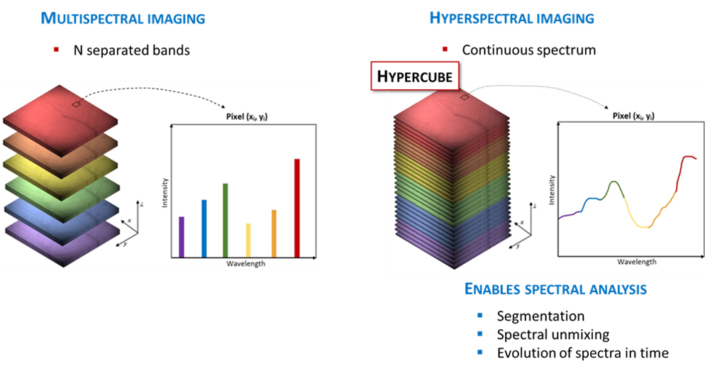
\includegraphics[width=0.7\linewidth]{media/images/hyperspectral_image.png}
    \caption{Esquemas para almacenar los valores de píxel reales de una imagen en un archivo \acrshort{bil}, referencia:\ \cite{Archivos82:online}}\ \label{fig:hyperspectral_image}
\end{figure}

\begin{code}[numbers=left]{title=Gráfico de velas de los outliers, label=code:plot-outliers}{Python}
def plots_outliers(outliers_df: pd.DataFrame, column=53):
    fig, axes = plt.subplots(ncols=2, figsize=(10, 5))
    sns.histplot(outliers_df[column], binwidth=1, ax=axes[0])
    sns.boxplot(outliers_df[column], ax=axes[1])
    fig.tight_layout()
    plt.show()
\end{code}

\begin{code}[numbers=left]{title=Detección de outliers utilizando \textit{zscore}, label=code:zscore}{Python}
...
    zscore = np.abs(stats.zscore(df))
    data_clean = df[(zscore < 3).all(axis=1)]
    df = data_clean
...
\end{code}

\begin{code}[numbers=left]{title=Gráfico de curvas de aprendizaje, label=code:plot-learning-curves}{Python}
def plots_balancing(df, df_balanced):
    fig, axis = plt.subplots(ncols=2, figsize=(10, 5))
    fig.suptitle(f'Balance of {src.utils.dev_config.OBJECTIVE_COLUMN}')
    axis[0].set_title(f'Before balancing {src.utils.dev_config.OBJECTIVE_COLUMN}')
    axis[1].set_title(f'After balancing {src.utils.dev_config.OBJECTIVE_COLUMN}')
    plot_balance(df, ax, 0)
    plot_balance(df_balanced, ax, 1)
    f.tight_layout()
    plt.show()
z

def plot_balance(df, axis, axis_number):
    return sns.histplot(df[src.utils.dev_config.OBJECTIVE_COLUMN], ax=axis[axis_number] if axis_number else axis)
\end{code}

\begin{code}[numbers=left]{title=Gráfico de comparación del balanceo, label=code:plots_balancing}{Python}
def plot_learning_curves(model, model_name, x, y):
    x_train, x_val, y_train, y_val = train_test_split(x, y, test_size=0.2)
    train_errors, val_errors = [], []
    
    for m in range(5, len(x_train)):
        model.fit(x_train[:m], y_train[:m])
        y_train_predict = model.predict(x_train[:m])
        y_val_predict = model.predict(x_val)
        train_errors.append(metrics.fbeta_score(y_train[:m], y_train_predict, beta=2))
        val_errors.append(metrics.fbeta_score(y_val, y_val_predict, beta=2))
        
    plt.title(f'{model_name} - Learning curves')
    plt.plot(np.sqrt(train_errors), "r-+", linewidth=2, label="train")
    plt.plot(np.sqrt(val_errors), "b-", linewidth=3, label="val")
    plt.xlabel("Training set size")
    plt.ylabel("f2 score")
    plt.legend(loc="best")
    plt.show()
\end{code}